\documentclass[openany,11pt]{book}
\usepackage[top=1in, bottom=1in,left=0.9in, right=0.9in]{geometry}
\usepackage{amsmath, amsthm, amssymb, amsfonts}
\usepackage{thmtools}
\usepackage{graphicx}
\usepackage{setspace}
\usepackage{bm}
\usepackage{extpfeil}
\usepackage{verbatim}
\usepackage{mathrsfs}
\usepackage{fontspec}
\usepackage{geometry}
\usepackage{float}
\usepackage{hyperref}
\hypersetup{
    colorlinks=true,
    linkcolor=blue,  % 修改为你想要的颜色
    citecolor=blue,   % 修改为你想要的颜色
    urlcolor=green   % 修改为你想要的颜色
}
\newcommand{\red}{\textcolor{red}}
\newcommand{\blue}{\textcolor{blue}}
\usepackage[utf8]{inputenc}
\usepackage[english]{babel}
\usepackage{framed}
\usepackage[dvipsnames]{xcolor}
\usepackage{tcolorbox}
\usepackage[UTF8]{ctex}
\usepackage{mathtools}
\colorlet{LightGray}{White!90!Periwinkle}
\colorlet{LightOrange}{Orange!15}
\colorlet{LightGreen}{Green!15}
\usepackage{graphicx}
\usepackage{caption}
\usepackage{wrapfig}
\usepackage{esint}
\usepackage{subcaption}
\newcommand{\HRule}[1]{\rule{\linewidth}{#1}}
\newcommand{\for}{\because}
\newcommand{\so}{\therefore}
\newcommand{\cz}{\exists \hspace{0.1cm}}
%\setmainfont{CMK.ttf}
\setCJKmainfont{CMK.ttf}

\newfontfamily{\CMK}{CMK.ttf}
\newenvironment{remark}[1][\textbf{Remark}]{
  \renewcommand{\proofname}{\fontsize{10pt}{11pt}\selectfont #1}%
  \begin{proof}
	\CMK\fontsize{10pt}{11pt}\selectfont 
  }{
	\end{proof}
}
\newenvironment{pf}[1][\textbf{Proof}]{
  \renewcommand{\proofname}{\fontsize{10pt}{11pt}\selectfont #1}%
  \begin{proof}
	\kaishu\fontsize{10pt}{11pt}\selectfont 
  }{
	\end{proof}
}
\declaretheoremstyle[name=Definition,]{thmsty}
\declaretheorem[style=thmsty,numberwithin=section]{definition}
\tcolorboxenvironment{definition}{colback=white}

\declaretheoremstyle[name=Theorem,]{thmsty}
\declaretheorem[style=thmsty,numberwithin=section]{theorem}
\tcolorboxenvironment{theorem}{colback=LightGray}

\declaretheoremstyle[name=Proposition,]{prosty}
\declaretheorem[style=prosty,numberlike=theorem]{proposition}
\tcolorboxenvironment{proposition}{colback=LightOrange}

\declaretheoremstyle[name=Corollary,]{prcpsty}
\declaretheorem[style=prcpsty,numberlike=theorem]{corollary}
\tcolorboxenvironment{principle}{colback=LightGreen}

\setstretch{1.2}
\geometry{
    textheight=9in,
    textwidth=5.5in,
    top=1in,
    headheight=12pt,
    headsep=25pt,
    footskip=30pt
}

% ------------------------------------------------------------------------------

\begin{document}

% ------------------------------------------------------------------------------
% Cover Page and ToC
% ------------------------------------------------------------------------------

\title{ \normalsize \textsc{}
		\\ [2.0cm]
		\HRule{1.5pt} \\
		\LARGE \textbf{\uppercase{Differential Geometry}
		\HRule{2.0pt} \\ [0.6cm] \LARGE{Lecture Notes} \vspace*{10\baselineskip}}
		}
\date{}
\author{\textbf{Collapsar} 
		\date{\today}}

\maketitle
\newpage

\tableofcontents
\newpage

% ------------------------------------------------------------------------------
\chapter{1}
\chapter{2}
\chapter{hh}
\chapter{ff}
\chapter{微分形式及其积分}

\section{微分形式}
\subsection{$l$形式}
如果 $(0,l)$ 型张量$\omega_{a_1\cdots a_l}\in \mathscr{T}_V(0,l)$满足
\begin{align}
    \omega_{a_1\cdots a_l}=\omega_{[a_1\cdots a_l]},
\end{align}
其中方括号表示“反对称”操作,称
$\omega_{a_1\cdots a_l}$ 为 $n$ 维矢量空间 $V$ 上的 \textcolor{blue}{$l$次形式}  (简称$l$形式,$l$-form).
为了书写方便,印刷体可以略去下标后加粗,将$l$形式记作 $\boldsymbol{\omega}$,手写体可以写作 $\underline{\omega}$.

对于如上的一个$l$形式,其在任意基底下的分量都满足类似的等式
\begin{align}
\omega_{\mu_1\cdots \mu_l}=\omega_{[\mu_1\cdots \mu_l]},
\end{align}
反过来,如果存在一个基底使得上式成立,那么一定会得到矢量空间 $V$ 上的该 $l$ 次形式$\boldsymbol{\omega}$.

\begin{remark}
由 $\boldsymbol{\omega}$ 的定义不难得到,$\omega_{[a_1\cdots a_l]}$ 中的偶排列项等于$\omega_{a_1\cdots a_l}$,奇排列项等于 $-\omega_{a_1\cdots a_l}$.对于“3形式”有$$\omega_{abc}=-\omega_{bac}=\omega_{bca}.$$

同时在 $l$ 形式的分量 $\omega_{\mu_1\cdots\mu_l}$ 中,凡是出现了重复指标者必为零,如对于“3形式”有 $\omega_{232}=0$.
\end{remark}

$V$上全体 $l$ 形式的集合记作 $\Lambda(l)$.由于$l$形式是 $(0,l)$ 型张量,则$\Lambda(l)$ 自然就是 $V$ 上 $(0,l)$ 型张量场$\mathscr{T}_V(0,l)$ 的子集.进一步可证明, $\Lambda(l)$ 是 $\mathscr{T}_V(0,l)$ 的线性子空间.

常见的两个l形式以及相应的 $\Lambda(l)$如下:
\begin{itemize}
\item 任一实数称为$V$上的0形式,则 $\Lambda(0)=\mathbb{R}$ ;
\item V上的对偶矢量,也就是(0,1)型张量是1形式,则 $\Lambda(1)=V^*$.
\end{itemize}

\begin{figure}[htbp]
    \centering
 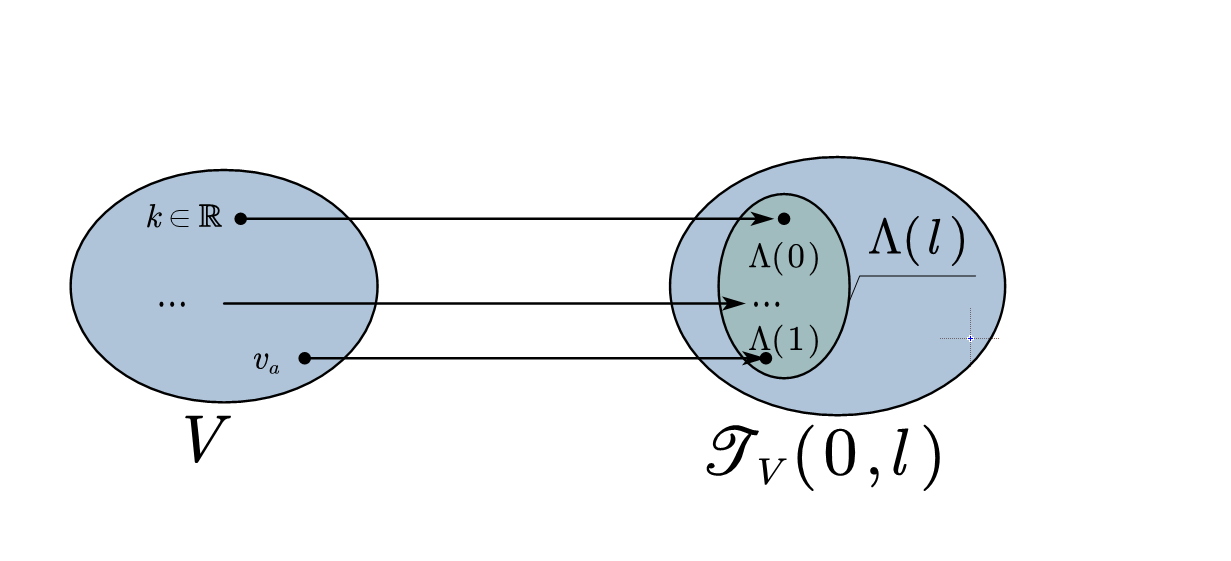
\includegraphics[width=\textwidth]{img/5-1.png}
    \caption{$\Lambda(l)$ 是 $V$ 上全体 $l$ 形式的集合}
\end{figure}
\subsection{楔形积}
假设$\boldsymbol{\omega}$ 和 $\boldsymbol{\mu}$ 分别是$l$形式和$m$形式,定义它们的\textcolor{blue}{楔形积} (简称楔积,wedge product)是如下定义的$l+m$形式:
\begin{align}
\boldsymbol{\omega}\wedge\boldsymbol{\mu}=(\omega \wedge\mu)_{a_1\cdots a_lb_1\cdots b_m}
=\omega_{a_1\cdots a_l} \wedge\mu_{b_1\cdots b_m}
:=\dfrac{(l+m)!}{l!m!}\omega_{[a_1\cdots a_l}\mu_{b_1\cdots b_m]}.
\end{align}

即映射 $\wedge:\Lambda(l)\times\Lambda(m)\to\Lambda(l+m)$.

楔形积满足如下性质:
\begin{align}
    \boldsymbol{\omega}\wedge\boldsymbol{\mu}&=(-1)^{lm}\boldsymbol{\mu}\wedge \boldsymbol{\omega},
\end{align}
\begin{align}
    \mathrm{dim}\Lambda(l)&=\left\{
        \begin{aligned}
    \dfrac{n!}{l!(n-l)!},l\leqslant n;\\
    \Lambda(l)=\{0\},l>n.
        \end{aligned}
    \right.
\end{align}
其中设$n=\mathrm{dim}V$.

\begin{remark}
以$n=3,l=2$为例说明.设 $\{(e_1)^a,(e_2)^a,(e_3)^a\}$ 是 $V$ 的基底,$\{(e^1)_a,(e^2)_a,(e^3)_a\}$ 为其对偶基底,则 $\omega_{ab}$可以展开为:
 $$
\begin{aligned}
\omega_{ab}&=\omega_{11}(e^1)_a(e^1)_b+\omega_{12}(e^1)_a(e^2)_b+\omega_{13}(e^1)_a(e^3)_b\\
&+\omega_{21}(e^2)_a(e^1)_b+\omega_{22}(e^2)_a(e^2)_b+\omega_{23}(e^2)_a(e^3)_b\\
&+\omega_{31}(e^3)_a(e^1)_b+\omega_{32}(e^3)_a(e^2)_b+\omega_{33}(e^3)_a(e^3)_b\\
\xlongequal{\omega_{\mu\mu}=0}&\omega_{12}(e^1)_a(e^2)_b+\omega_{13}(e^1)_a(e^3)_b+\omega_{21}(e^2)_a(e^1)_b\\
+&\omega_{23}(e^2)_a(e^3)_b+\omega_{31}(e^3)_a(e^1)_b+\omega_{32}(e^3)_a(e^2)_b\\
\xlongequal {\omega_{\mu\nu}=-\omega_{\nu\mu}}&\omega_{12}
\underset{(e^1)_a\wedge (e^2)_b}{\underbrace{[(e^1)_a(e^2)_b-(e^2)_a(e^1)_b]}}+\omega_{13}\underset{(e^1)_a\wedge (e^3)_b}{\underbrace{[(e^1)_a(e^3)_b-(e^3)_a(e^1)_b]}}\\
&+\omega_{23}\underset{(e^2)_a\wedge (e^3)_b}{\underbrace{[(e^2)_a(e^3)_b-(e^3)_a(e^2)_b]}}=\sum\limits_C \omega_{\mu\nu}(e^\mu)_a\wedge(e^\nu)_b.
\end{aligned}$$

以上表明,任一 $\omega_{ab}\in \Lambda(2)$ 可以用括号下面的三个2形式线性表出,而且这三个2形式彼此线性独立.因此 $\mathrm{dim}\Lambda(2)=3$.由此进一步推广到 $l,n\in \mathbb{N}^+,l\leqslant n$的情况:
$$\omega_{a_1\cdots a_l}=\sum\limits_C\omega_{\mu_1\cdots\mu_l}(e^{\mu_1})_{a_1}\wedge\cdots\wedge(e^{\mu_l})_{a_l},$$
其中,$\{(e^1)_a,\cdots,(e^n)_a\}$为$V^*$的基底,$\sum\limits_C$表示对 $n$ 个数 $1,2,\cdots,n$ 中取 $l$ 个的各种组合求和,且
$$\omega_{\mu_1\cdots\mu_l}=\omega_{a_1\cdots a_l}(e_{\mu_1})^{a_1}\cdots(e_{\mu_l})^{a_l}.$$
\end{remark}

对流形 $M$ 或者 $A\subset M$的任一点 $p$ 都指定 $V_p$ 上的一个 $l$ 形式,就得到了流形 $M$ 或者 $A$ 上的一个 $l$ 形式场.$M$ 上的光滑 $l$ 形式场称为 \blue{$l$次微分形式场}(differential l-form),简称$l$形式场或$l$形式.

在流形M上选定坐标系$\{O,\psi\}$,将基底 $\{(e^\mu)_a\}$具体选为对偶坐标基底 $\{(\mathrm{d}x^\mu)_a\}$,于是就有
\begin{align}
\displaystyle\omega_{a_1\cdots a_l}=\sum\limits_C\omega_{\mu_1\cdots\mu_l}
(\text{d}x^{\mu_1})_{a_1}\wedge\cdots\wedge(\text{d}x^{\mu_l})_{a_l},
\end{align}
其中,$\omega_{\mu_1\cdots\mu_l}=\omega_{a_1\cdots a_l}\left(\dfrac{\partial}{\partial x^{\mu_1}}\right)^{a_1}\cdots\left(\dfrac{\partial}{\partial x^{\mu_l}}\right)^{a_l}$是$O$上的函数.
\begin{remark}
当$l=n$时,$\sum\limits_C$是对 $n$ 个数 $1,2,\cdots,n$ 中取 $n$ 个的各种组合求和,只有唯一一项,因此有
$$
\begin{aligned}
&\omega_{a_1\cdots a_n}=\omega_{1\cdots n}(\text{d}x^{1})_{a_1}\wedge\cdots\wedge(\text{d}x^{n})_{a_n}.\\
&\Rightarrow \boldsymbol{\omega}=\omega_{1\cdots n}(\text{d}x^{1})\wedge\cdots\wedge(\text{d}x^{n})\\
&=\underset{M\text{上的标量场}}{\underbrace{\omega_{1\cdots n}(x^1,\cdots,x^n)}}(\text{d}x^{1})\wedge\cdots\wedge(\text{d}x^{n}).
\end{aligned}$$
以上表明,流形 $M$ 上任一点 $p$ 上的所有 $n$ 形式的集合 $\Lambda_M(n)$是一维向量空间.
\end{remark}
\subsection{外微分算符}

流形 M 上的\blue{外微分算符}(exterior differentiation operator)定义为
\begin{align}
(\mathrm{d}\omega)_{ba_1\cdots a_l}:=(l+1)\nabla_{[b}\omega_{a_1\cdots a_l]},
\end{align}
即 $\mathrm{d}$ 是一个映射:
$\Lambda_M(l)\xrightarrow [\text{外微分}]{\mathrm{d}} \Lambda_M(l+1)$.

对于0形式场的 $f$,根据上述外微分的定义有有$(\mathrm{d}f)_b=\nabla_bf$,这与之前的定义是一致的.
\begin{remark}
定义中 $\nabla_b$可为任一导数算符.这是因为
$$
\begin{aligned}
\tilde{\nabla}_{[b}\omega_{a]}=\nabla_{[b}\omega_{a]}+C^c{}_{[ba]}\omega_c=\nabla_{[b}\omega_{a]}+C^c{}_{[(ba)]}\omega_c=\nabla_{[b}\omega_{a]}.
\end{aligned}
$$
可见定义外微分算符并不要指定导数算符,更无需对流形附加额外的结构.
\end{remark}


外微分具有如下性质:
\begin{enumerate}
\item 当 $\boldsymbol{\omega}$ 以对偶坐标基底展开时,外微分 $\mathrm{d}$ 对它的作用表现为$\mathrm{d}$直接作用于$\boldsymbol{\omega}$ 在该基底下的分量,即
$$
\begin{aligned}
\omega_{a_1\cdots a_l}=\sum\limits_C&\omega_{\mu_1\cdots\mu_l}(\text{d}x^{\mu_1})_{a_1}\wedge\cdots\wedge(\text{d}x^{\mu_l})_{a_l}.\\
\Rightarrow (\text{d}\omega)_{ba_1\cdots a_l}&=\sum\limits_C(\text{d}\omega_{\mu_1\cdots\mu_l})_b(\text{d}x^{\mu_1})_{a_1}\wedge\cdots\wedge(\text{d}x^{\mu_l})_{a_l}.
\end{aligned}
$$
\item $\mathrm{d}\circ \mathrm{d}=0$.

\begin{proof}
    $[\mathrm{d}(\mathrm{d}\omega)]_{cba_1\cdots}=(l+2)(l+1)\nabla_{[c}\nabla_{[b}\omega_{a_1\cdots]]}=(l+2)(l+1)\partial_{[(c}\partial_{b)}\omega_{a_1\cdots]}=0.
$
\end{proof}
\item 设$\boldsymbol{\omega}$为流形$M$的 $l$形式场,若$\mathrm{d}\boldsymbol{\omega}=0$,称 $\boldsymbol{\omega}$是\blue{闭的}(closed);若存在$l-1$形式场 $\boldsymbol{\mu}$,使得$\boldsymbol{\omega}=\mathrm{d}\boldsymbol{\mu}$,称$\boldsymbol{\omega}$是\blue{恰当的}(exact).
若$\boldsymbol{\omega}$是恰当的,则一定是闭的,但逆命题不一定成立.
\end{enumerate}
\begin{remark}
逆命题成立需对流形提出一些要求,平凡流形$\mathbb{R}^n$符合这个要求,而流形一定是局域平凡的,因此任意流形上闭的 $l$形式场至少是局域恰当的.用数学语言表述就是:

设$\boldsymbol{\omega}$ 是流形M上的闭的$l$形式场,则$\forall p\in M,$必有邻域$N$,在其上存在$l-1$形式场$\boldsymbol{\mu}$,使得$\boldsymbol{\omega}=\mathrm{d}\boldsymbol{\mu}$. 

在流形M上未必存在满足条件的$\boldsymbol{\mu}$,但在每点的邻域上却存在.但是不能这样理解,仅在某确定的p点附近存在相应的$\boldsymbol{\mu}$,其余位置不存在. 
\end{remark}

\section{流形上的积分}

计算任意流形上的积分,首先必须对流形进行“定向”.$n$ 维流形上若存在一个 $C^0$而且处处不为0的$n$形式场 $\boldsymbol{\varepsilon}$,就说该流形是\blue{可定向的}(orientable).确定了满足上述条件的 $\boldsymbol{\varepsilon}$后,流形M则是已定向的.

\begin{remark}
常见的$\mathbb{R}^3$是可以定向的,因为其上存在$C^\infty$的3形式场 $\boldsymbol{\varepsilon}\equiv\mathrm{d}x\wedge\mathrm{d}y\wedge\mathrm{d}z$.
常见的不可定向流形如莫比乌斯带.
\end{remark}
设$\boldsymbol{\varepsilon^\prime}$与$\boldsymbol{\varepsilon}$都是$C^0$而且处处非零的n形式场,并且满足$\boldsymbol{\varepsilon^\prime}=h\boldsymbol{\varepsilon}$,当函数$h>0$时,称$\boldsymbol{\varepsilon^\prime}$与$\boldsymbol{\varepsilon}$为等价的定向,它们给出M的同一个定向.
\begin{remark}
事实上,对于连通的流形,$h$在M上恒正或者恒负.

由于n维流形M上每点的全体n形式的集合是一个一维矢量空间,则任意两个n形式场$\boldsymbol{\varepsilon},\boldsymbol{\varepsilon^\prime}$必定线性相关,即存在$h$使得$\boldsymbol{\varepsilon^\prime}=h\boldsymbol{\varepsilon}$.当$\boldsymbol{\varepsilon},\boldsymbol{\varepsilon^\prime}$为$C^0$时,$h$自然也是$C^0$的.由$\boldsymbol{\varepsilon},\boldsymbol{\varepsilon^\prime}$处处非零可知,$h$只能恒正或者恒负. 
\end{remark}

在流形M上选好以$\boldsymbol{\varepsilon}$为代表的定向,设开域$O\subset M,$且其上存在处处为正的函数$h$使得$\boldsymbol{\varepsilon}=h(e^1)_{a_1}\wedge\cdots\wedge(e^n)_{a_n},$ 其中$\{(e^\mu)_a\}$是$O$上的基底场$\{(e_\mu)^a\}$的对偶基,则称$\{(e_\mu)^a\}$是\blue{右手的}(right handed),该坐标系称为\blue{右手坐标系}.
\begin{remark}
    反之,若$h<0$,$O$上的基地场$\{(e_\mu)^a\}$称为左手的,该坐标系称为左手系.
\end{remark}
\begin{figure}[htbp]
    \centering
 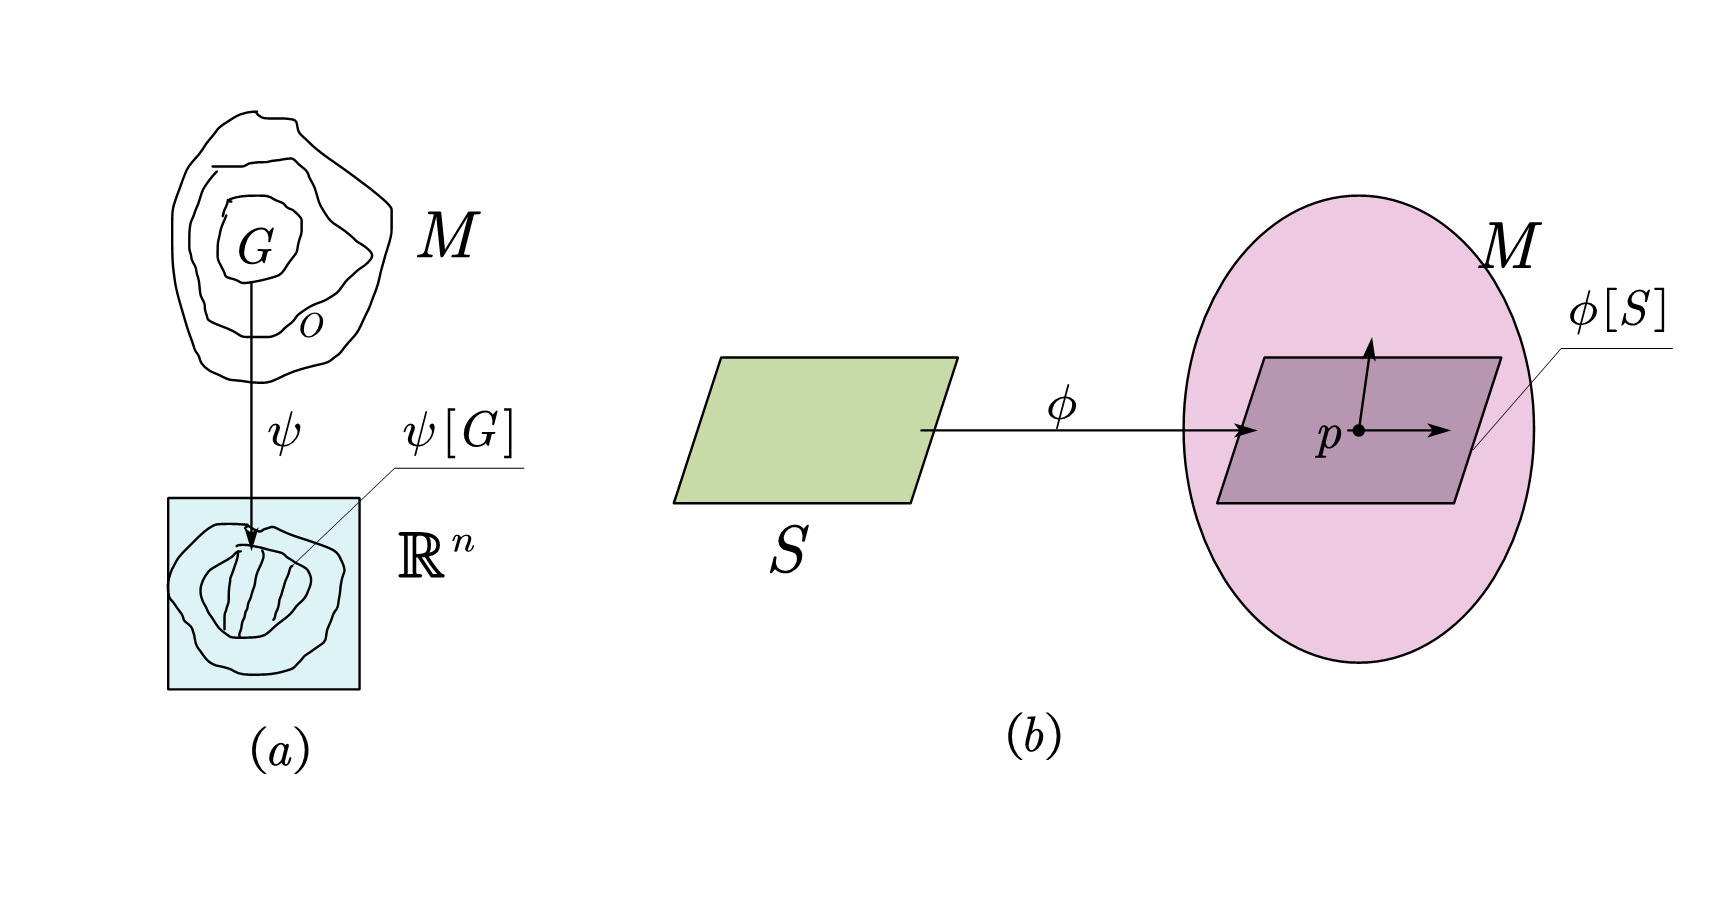
\includegraphics[width=\textwidth]{img/5-2.png}
    \caption{(a):流形上积分的定义,(b):n=2的情况}
    \label{fig:5-2}
\end{figure}
由于$\boldsymbol{\omega}$可以对偶坐标基矢的楔形积表示为:
\begin{align}
\boldsymbol{\omega}=\underset{M\text{上的标量场或者n元函数}}{\underbrace{\omega_{1\cdots n}(x^1,\cdots,x^n)}}(\text{d}x^{1})\wedge\cdots\wedge(\text{d}x^{n}),
\end{align}
所以$\boldsymbol{\omega}$在流形$G\subset M$上的积分自然可以定义为$\boldsymbol{\omega}$在该对偶坐标基矢下的分量$\omega_{1\cdots n}$,作为一个n元函数,在$G\subset M$的像$\psi[G]\subset \mathbb{R}^n$上的普通Riemann或者Lebesgue积分,即(如上图(a)所示)
\begin{align}
 \int_G \boldsymbol{\omega}:=\int_{\psi[G]}\omega_{1\cdots n}(x^1,\cdots,x^n)\mathrm{d}x^1\mathrm{d}x^2\cdots \mathrm{d}x^n,
\end{align}
其中$(O,\psi)$是$n$维定向流形M的右手坐标系.
\begin{remark}
以$n=2$为例,说明$\boldsymbol{\omega}$在$G$上的积分与所选的右手坐标系无关.

假设$(O,\psi),(O^\prime,\psi^\prime)$为右手坐标系且$G\subset O\cap O^\prime$,两系坐标记作$x^1,x^2;x^{1\prime},x^{2\prime}$,所以
$$\boldsymbol{\omega}=\omega_{12}\mathrm{d}x^1\wedge \mathrm{d}x^2=\omega_{12}^\prime\mathrm{d}x^{1\prime}\wedge \mathrm{d}x^{2\prime}.
$$
记
$$
\begin{aligned}
\int_G \boldsymbol{\omega}=\int_{\psi{[G]}}\omega_{12} \mathrm{d}x^1\mathrm{d}x^2,\left(\int_G \boldsymbol{\omega}\right)^\prime &=\int_{\psi^\prime{[G]}}\omega_{12}^\prime \mathrm{d}x^{1\prime}\mathrm{d}x^{2\prime},
\end{aligned}
$$
由于
$$
\begin{aligned}
\omega_{12}^\prime&=\dfrac{\partial x^\mu}{\partial x^{\prime 1}}\dfrac{\partial x^\nu}{\partial x^{\prime2}}\omega_{\mu\nu}=\dfrac{\partial x^1}{\partial x^{\prime 1}}\dfrac{\partial x^2}{\partial x^{\prime2}}\omega_{12}+\dfrac{\partial x^2}{\partial x^{\prime 1}}\dfrac{\partial x^1}{\partial x^{\prime2}}\omega_{21}\\
&=\omega_{12}\left(\dfrac{\partial x^1}{\partial x^{\prime 1}}\dfrac{\partial x^2}{\partial x^{\prime2}}-\dfrac{\partial x^2}{\partial x^{\prime 1}}\dfrac{\partial x^1}{\partial x^{\prime2}}\right)\\
&=\omega_{12}\mathrm{det}\left(\dfrac{\partial x^\mu}{\partial x^{\prime\nu}}\right)=\omega_{12}J,
\end{aligned}
$$
为确保上式对$\{x\},\{x^\prime\}$分别是右、左手系的情况也成立,应该进一步改写为$
\omega_{12}^\prime=\omega_{12}|J|,
$
根据二重积分的换元公式,有
$$
\int_{\psi[G]}\omega_{12}\mathrm{d}x^1\mathrm{d}x^2=\int_{\psi^\prime[G]}\omega_{12}|J|\mathrm{d}x^{1\prime}\mathrm{d}x^{2\prime}=\int_{\psi^\prime[G]}\omega_{12}^\prime\mathrm{d}x^{1\prime}\mathrm{d}x^{2\prime}.
$$
\end{remark}

如图\ref{fig:5-2}(b)所示,设$S,M$分别是$l,n$维流形,且$l<n$,则$\phi:S\to M$是嵌入的.$\phi[S]$上的$l$形式场$\boldsymbol{\mu}$ “切于”
$\phi[S]$,若$\boldsymbol{\mu}|_{q}\in W_q,\forall q\in \phi[S]$,即$\boldsymbol{\mu}$是将$W_q$的任意$l$个元素变为一个实数的线性映射.只有“切于”$\phi[S]$的$\boldsymbol{\mu}$的积分在上述定义下才有意义.对于不“切于”$\phi[S]$的$\boldsymbol{\mu}$,只需要将其作用范围限制在$W_p$,并且记作$\tilde{\mu}$.具体定义如下:

设$\boldsymbol{\mu}_{a_1\cdots a_l}$是$l$维子流形$\phi[S]\subset M$上的$l$形式场.将$\phi[S]$视为脱离M而独立存在的流形,其上的$l$形式$\tilde{\boldsymbol{\mu}}_{a_1\cdots a_l}$称为${\mu}_{a_1\cdots a_l}$在$\phi[S]$上的限制,若
$\forall q\in \phi[S],(\omega_1)^a,\cdots,(\omega_l)^a\in W_q$有
\begin{align}
\tilde{\boldsymbol{\mu}}_{a_1\cdots a_l}|_q(\omega_1)^{a_1}\cdots(\omega_l)^{a_l}=\boldsymbol{\mu}_{a_1\cdots a_l}|_q(\omega_1)^{a_1}\cdots(\omega_l)^{a_l}.\end{align}
\section{Stokes公式}

\textcolor{blue}{$n$维带边流形}(manifold with boundary)类似于$n$维流形,具体而言就是$N$的开覆盖$\{O_\alpha\}$的每一元素$O_\alpha$都应该同胚于$\mathbb{R}^{n-}$的一个开子集,$N$中全体被映射到$x^1=0$处的点组成$N$的\textcolor{blue}{边界},记作$\partial N$. $\partial N$是$n-1$维流形,$i(N)\equiv N-\partial N$是$n$维流形(如图\ref{fig:5-3}(a)所示).
\begin{remark}
    最简单的带边流形的例子是$$\mathbb{R}^{n-}:=\{(x^1,\cdots,x^n)\in \mathbb{R}^n|x^1\leqslant 0\},$$
    $x^1,\cdots,x^n$是自然坐标,$x^1=0$的所有点组成的子集是$\mathbb{R}^{n-}$的边界,而$\mathbb{R}^{n-}$自身则是$n-1$维流形.
\end{remark}
\begin{figure}[htbp]
    \centering
 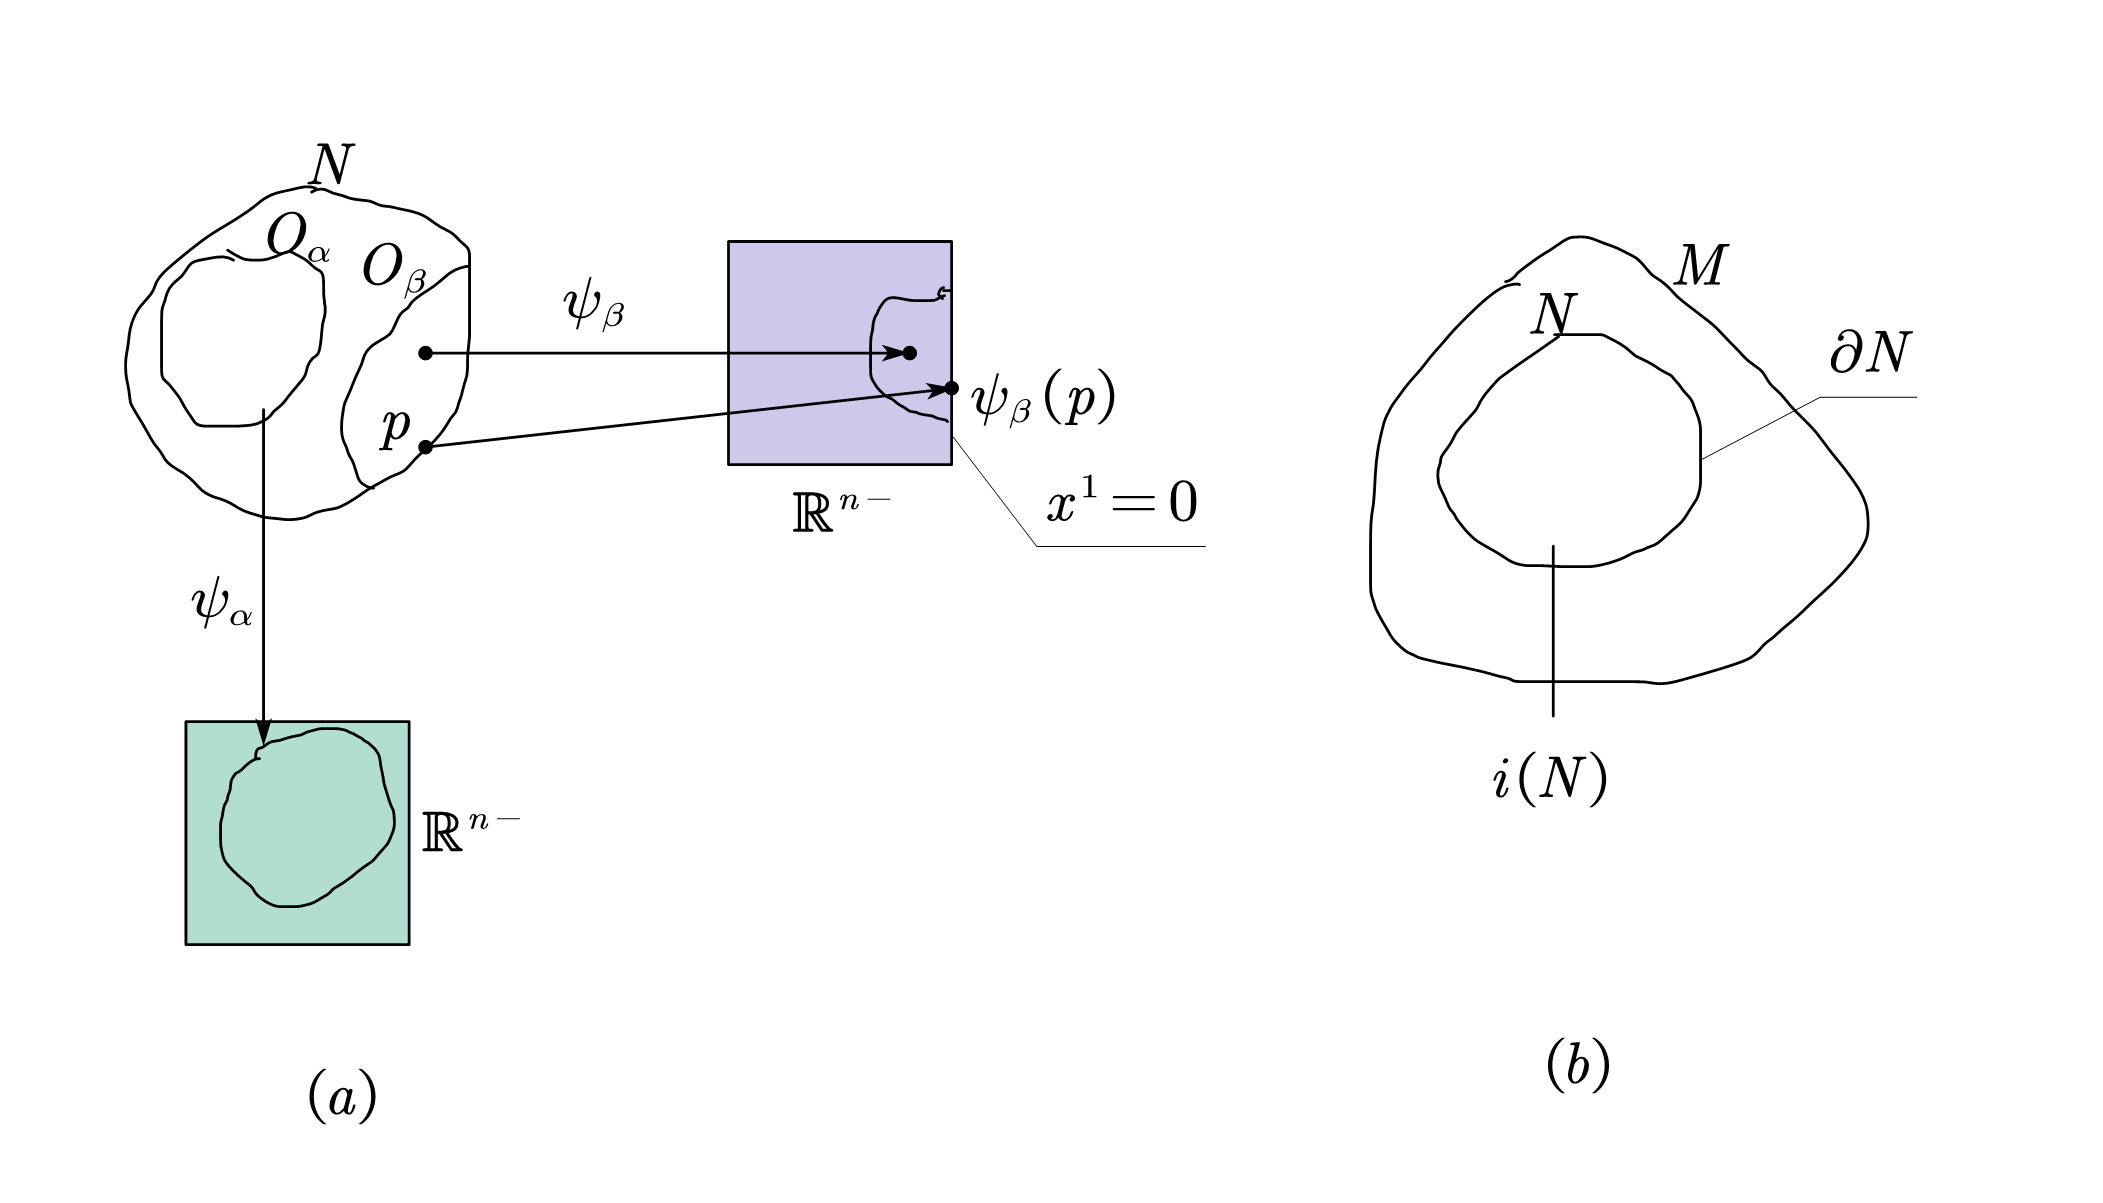
\includegraphics[width=\textwidth]{img/5-3.png}
    \caption{(a):带边流形$N$的示意图,$p$为边界点,(b):$Stokes$定理的示意图}
    \label{fig:5-3}
\end{figure}
如图\ref{fig:5-3}(b)所示,设$n$维定向流形$M$的紧致子集$N$是一个$n$维带边流形,$\boldsymbol{\omega}$是$M$上的至少$c^1$可微的$n-1$形式场,则有$Stokes$定理如下:
\begin{align}
\boxed{\int_{i(N)}\mathrm{d}\boldsymbol{\omega}=\int_{\partial N}\boldsymbol{\omega}.}
\end{align}
\begin{remark}
    设$\boldsymbol{\varepsilon}$是$M$上的定向限制在$N$上得到的定向,它在$\partial N$上自然诱导出一个定向,记作$\overline{\boldsymbol{\varepsilon}}$.
    $Stokes$定理左边是$n$形式场$\mathrm{d}\boldsymbol{\omega}$在$n$维流形$i(N)$上(以$\boldsymbol{\varepsilon}$为定向)上的积分,右边是$n-1$形式场$\boldsymbol{\omega}$在$n-1$维流形$\partial N$(以$\overline{\boldsymbol{\varepsilon}}$为定向)上的积分.
\end{remark}
\begin{remark}
\begin{figure}[htbp]
    \centering
 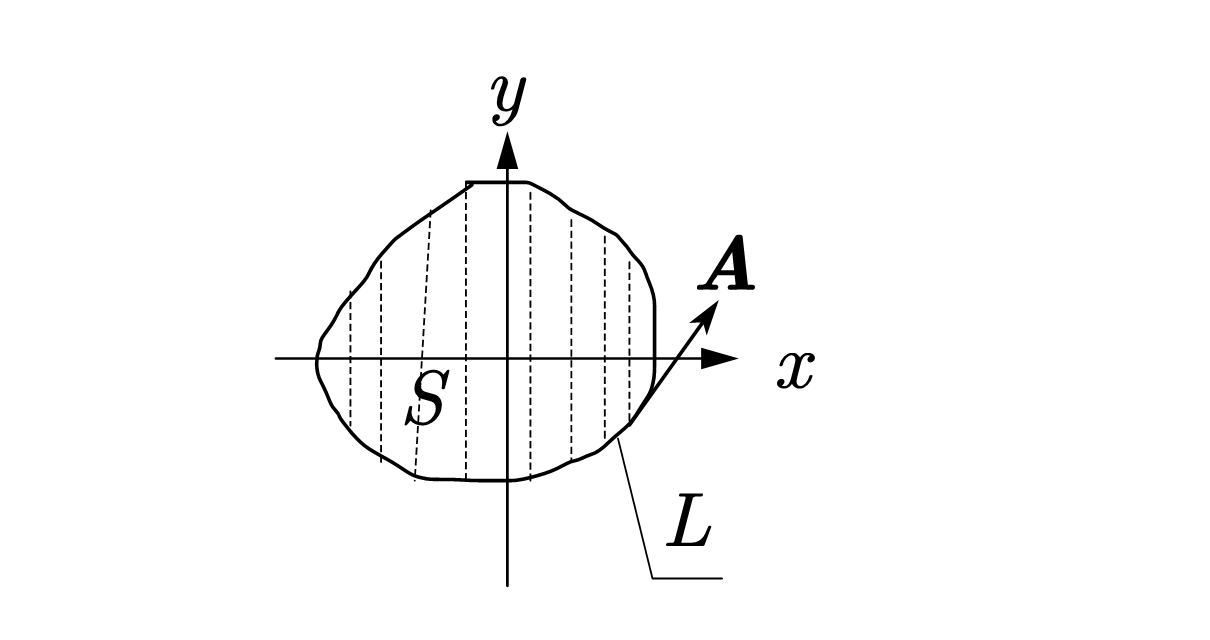
\includegraphics[width=0.8\textwidth]{img/5-4.png}
    \caption{二维欧氏空间的$Stokes$公式——$Green$公式}
    \label{fig:5-4}
\end{figure}
如图\ref{fig:5-4},设$\boldsymbol{A}$是二维欧氏空间的矢量场,$L$是$\mathbb{R}^2$中的光滑闭合曲线,$S$是由$L$包围的开子集,$x^1,x^2$为笛卡尔坐标,则有二维欧氏空间的$Stokes$公式,即$Green$公式如下:
$$
\iint_S\left(\dfrac{\partial A_2}{x^1}-\dfrac{A_1}{x^2}\right)\mathrm{d}x^1\mathrm{d}x^2=\oint_LA_l\mathrm{d}l.$$

此时,$i(N)=S,\partial N=L,N=S\cup L,M=\mathbb{R}^2.$
由于$$\boldsymbol{\omega}_a\equiv A_a\equiv \delta_{ab}A^b=A_\mu(\mathrm{d}x^\mu)_a,$$
所以有
$$
\begin{aligned}
\mathrm{d}\boldsymbol{\omega}=\mathrm{d}A_\mu\wedge\mathrm{d}x^\mu
&=\dfrac{\partial A_\mu}{\partial x^\nu}\mathrm{d}x^\nu\wedge \mathrm{d}x^\mu\\
&=\dfrac{\partial A_1}{\partial x^2}\mathrm{d}x^2\wedge \mathrm{d}x^1+\dfrac{\partial A_2}{\partial x^1}\mathrm{d}x^1\wedge \mathrm{d}x^2\\
&=\left(\dfrac{\partial A_2}{\partial x^1}-\dfrac{\partial A_1}{\partial x^2}\right)\mathrm{d}x^1\wedge \mathrm{d}x^2.
\end{aligned}
$$
从而$Green$公式的左边就可以写成$\displaystyle\int_{i(N)}\mathrm{d}\boldsymbol{\omega}.$

设$\tilde{\boldsymbol{\omega}}$是对$\boldsymbol{\omega}$进行的限制.选取线长$l$为$L$的局部坐标系,将$\tilde{\boldsymbol{\omega}}$以坐标基矢进行展开,则有
$$\tilde{\boldsymbol{\omega}}_a=\tilde{\boldsymbol{\omega}}_1(l)(\mathrm{d}l)_a.$$

上式两边同时和$\left(\dfrac{\partial}{\partial l}\right)^a$进行缩并,有
$$
\tilde{\omega}_1(l)=\tilde{\boldsymbol{\omega}}_a\left(\dfrac{\partial}{\partial l}\right)^a=\boldsymbol{\omega}_a\left(\dfrac{\partial}{\partial l}\right)^a=A_a\left(\dfrac{\partial}{\partial l}\right)^a=A_l,
$$
从而有$\tilde{\boldsymbol{\omega}}=A_l\mathrm{d}l$,于是
$$
\int_{\partial N}\boldsymbol{\omega}=\int_{\partial N}\tilde{\boldsymbol{\omega}}=\oint_{L}A_l\mathrm{d}l.
$$
由此可知,$Green$公式是$Stokes$公式在二维情况下的特例.
\end{remark}
\newpage
\section{体元}

$n$维可定向流形$M$上的任一个$C^0$而且处处非零的$n$形式场$\boldsymbol{\varepsilon}$,称为一个\textcolor{blue}{体元}.

\begin{remark}
    设$\boldsymbol{\varepsilon}_1,\boldsymbol{\varepsilon}_2$是两个$C^0$且处处不为零的$n$形式场,且有处处为正的函数$h$使得$\boldsymbol{\varepsilon}_1=h\boldsymbol{\varepsilon}_2,$那么$\boldsymbol{\varepsilon}_1,\boldsymbol{\varepsilon}_2$是两个不同的体元,但却代表同一个定向.对于连通流形,体元有无数个,定向却只有两个.
\end{remark}
定向流形上的积分和体元无需要求流形上附加度规结构.但是若流形上给定了度规场,就存在一个特定的体元.设$\boldsymbol{\varepsilon}_{a_1\cdots a_n}$是任一体元,则$\boldsymbol{\varepsilon}^{a_1\cdots a_n}=g^{a_1b_1}g^{a_2b_2} \cdots g^{a_nb_n}\boldsymbol{\varepsilon}_{b_1\cdots b_n}$,定义
\begin{align}
\boldsymbol{\varepsilon}^{a_1\cdots a_n}\boldsymbol{\varepsilon}_{a_1\cdots a_n}=(-1)^sn!(\varepsilon_{1\dots n})^2,
\end{align}
其中${\varepsilon}_{1\dots n}$是$\boldsymbol{\varepsilon}_{a_1\cdots a_n}$在正交归一基底的分量,$s$是$g_{ab}$在正交归一基底的分量中-1的个数.“度规选定一个特定的体元”,就是说规定体元$\boldsymbol{\varepsilon}_{a_1\dots a_n}$在正交归一基$\{(e^\mu)_a\}$的分量满足
\begin{align}
\boldsymbol{\varepsilon}_{a_1\cdots a_n}=\pm (e^1)_{a_1}\wedge\cdots \wedge (e^n)_{a_n}\Rightarrow \varepsilon_{1\cdots n}=\pm 1,
\end{align}
于是就有
\begin{align}
\boldsymbol{\varepsilon}^{a_1\cdots a_n}\boldsymbol{\varepsilon}_{a_1\cdots a_n}=(-1)^sn!,
\end{align}
满足上式的$\boldsymbol{\varepsilon}_{a_1\cdots a_n}$称为\textcolor{blue}{与度规$g_{ab}$相适配(相容)的体元}.“+”“-”分别表示右手和左手正交归一基.
\begin{remark}
    度规和体元只能将体元确定到相差一个负号的程度,若要唯一确定一个体元,还需加上“体元与定向相容”的条件,即代表体元的$\boldsymbol{\varepsilon}$与代表定向的$\boldsymbol{\varepsilon}$之间的乘子为正.
\end{remark}

设$\boldsymbol{\varepsilon}$是适配体元,$\{(e_\mu)^a\},\{(e^\mu)_a\}$为基底及其对偶基底,$g$为$g_{ab}$在此基底的分量组成的行列式,$|g|$为$g$的绝对值,则有
\begin{align}
\boldsymbol{\varepsilon}_{a_1\cdots a_n}=\pm\sqrt{|g|} (e^1)_{a_1}\wedge\cdots \wedge (e^n)_{a_n}.
\end{align}

\begin{remark}
    对于正交归一基底有$g$=1.
\end{remark}
设$\nabla_a,\boldsymbol{\varepsilon}$分别是与度规适配的导数算符和体元,则有
\begin{align}
\nabla_b\boldsymbol{\varepsilon}_{a_1\cdots a_n}=0.
\end{align}

关于体元,有如下恒等式
\begin{align}
    &\delta^{[a_1}{}_{a_1}\cdots \delta^{a_j}{}_{a_j}\delta^{a_{j+1}}{}_{b_{j+1}}\cdots \delta^{a_n]}{}_{b_n}=\dfrac{(n-j)!j!}{n!}\delta^{[a_{j+1}}{}_{b_{j+1}}\cdots \delta^{a_n]}{}_{b_n}.\\
    &\boldsymbol{\varepsilon}^{a_1\cdots a_n}\boldsymbol{\varepsilon}_{b_1\cdots b_n}=(-1)^sn!\delta^{[a_1}{}_{b_1}\cdots\delta^{a_n]}{}_{b_n}.\\
    &\boldsymbol{\varepsilon}^{a_1\cdots a_ja_{j+1}\cdots a_n}\boldsymbol{\varepsilon}_{a_1\cdots a_j b_{j+1}\cdots b_n=(-1)^s(n-j)!j!\delta^{[a_1}{}_{b_{j+1}}}\cdots \delta^{a_n]}{}_{b_n}.
\end{align}

\section{函数在流形上的积分,$Gauss$定理}

设$\boldsymbol{\varepsilon}$是流形$M$上的任一体元,$f$为$M$上的$C^0$函数,则\textcolor{blue}{$f$在$M$上的积分}$\displaystyle \int_M f$定义为$n$形式场$f\boldsymbol{\varepsilon}$在$M$上的积分,即
\begin{align}
\int_Mf:=\int_M f\boldsymbol{\varepsilon}.
\end{align}
\begin{remark}
\begin{figure}[htbp]
    \centering
 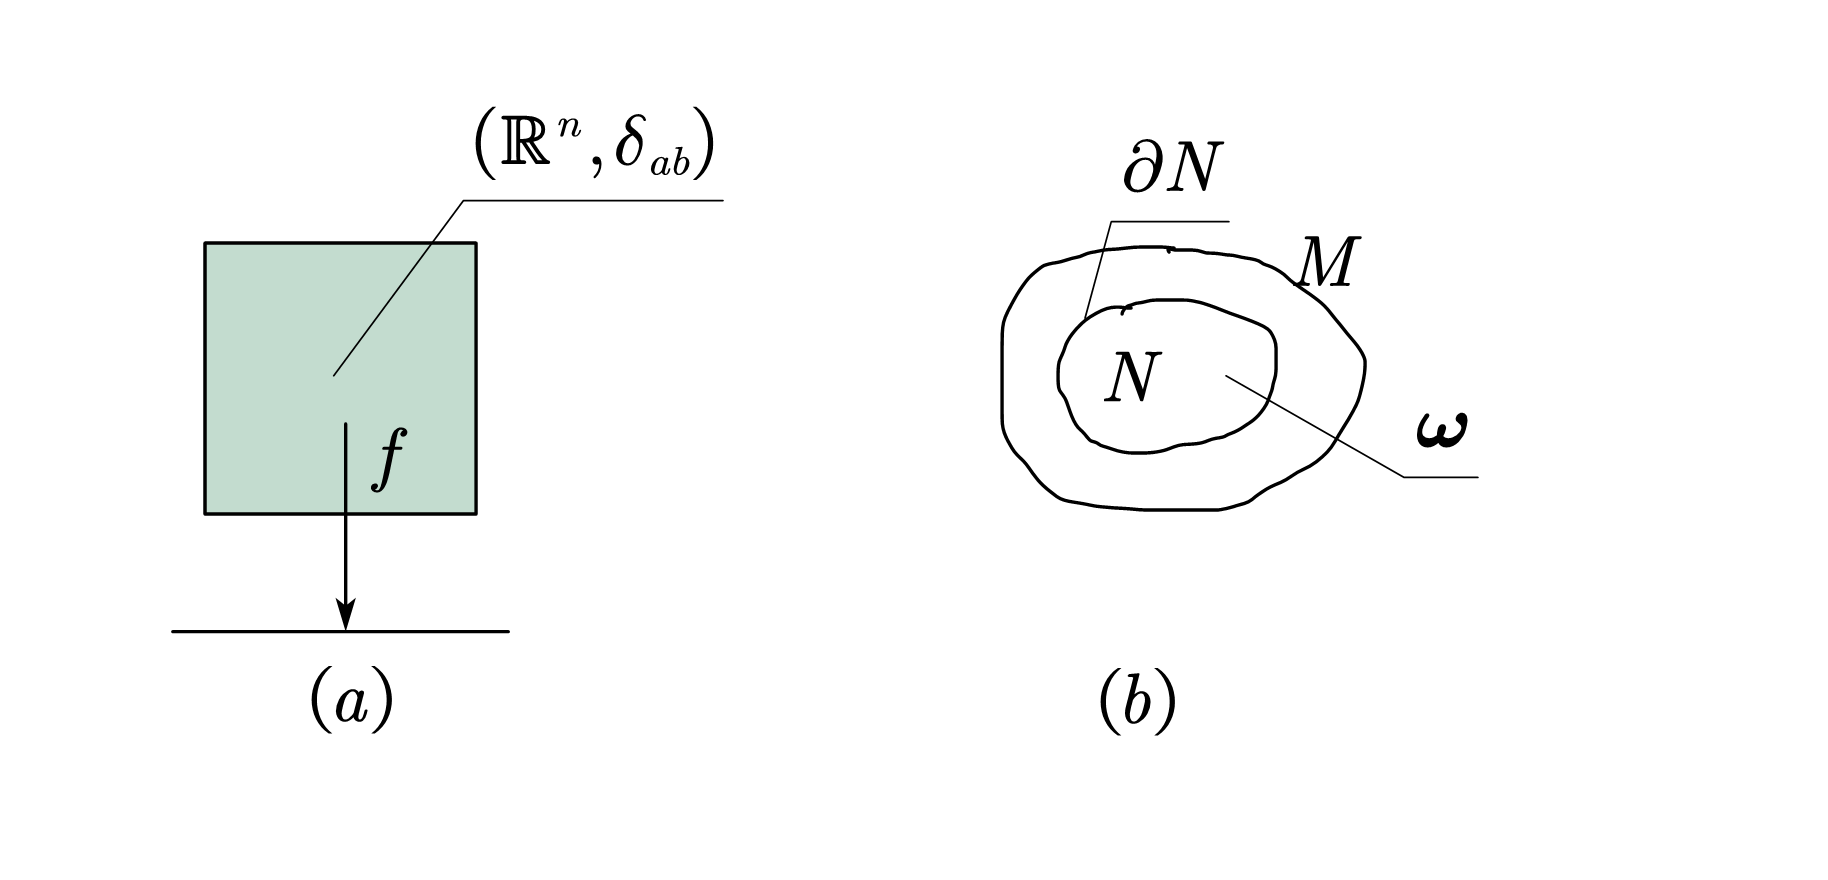
\includegraphics[width=\textwidth]{img/5-5.png}
    \caption{(a):三维欧氏空间的例子(b):式的示意图}
    \label{fig:5-5}
\end{figure}

如图\ref{fig:5-5}(a)所示,以三维欧氏空间$(\mathbb{R}^3,\delta_{ab})$为例说明上面定义的合理性.设$\{x,y,z\}$为右手笛卡尔坐标系,则相应的适配体元为$\boldsymbol{\varepsilon}=\mathrm{d}x\wedge\mathrm{d}y\wedge\mathrm{d}z$,于是$(\mathbb{R}^3,\delta_{ab})$上的函数$f:\mathbb{R}^3\to\mathbb{R}$的积分按照上面的定义就是
$$
\int_{\mathbb{R}^3}f=\int_{\mathbb{R}^3}f\boldsymbol{\varepsilon}=\int_{\mathbb{R}^3}\boldsymbol{\omega}=\iiint F(x,y,z)\mathrm{d}x\mathrm{d}y\mathrm{d}z,
$$
其中$F(x,y,z)$是$f$与笛卡尔坐标系$\{x,y,z\}$结合而得到的三元函数.

若采用球坐标系,则线元可以表示为$$
\mathrm{d}s^2=\mathrm{d}r^2+r^2(\mathrm{d}\theta^2+\sin^2\theta\mathrm{d}\varphi^2),
$$
于是就有度规$g_{ab}$的在球坐标系基底下的分量的行列式$g$为
$$g=\begin{vmatrix}
    1 & 0&0 \\
    0 & r^2&0\\
    0 & 0&r^2\sin\theta
    \end{vmatrix}=r^4\sin^2\theta>0,$$
    于是就有$$
    \boldsymbol{\omega}=r^2\sin\theta \mathrm{d}r\wedge \mathrm{d}\theta\wedge\mathrm{d}\varphi,
    $$
   从而
   $$\int f=\int f\boldsymbol{\varepsilon}=\int\boldsymbol{\omega}=\iiint\hat{F}(r,\theta,\varphi)r^2\sin\theta\mathrm{d}r\mathrm{d}\theta\mathrm{d}\varphi,$$
   其中$\hat{F}(r,\theta,\varphi)$是$f$与球坐标系$\{r,\theta,\varphi\}$结合而得到的三元函数.
\end{remark}
如图\ref{fig:5-5}(b)所示,设$M$是$n$维定向流形,$N$是其中的$n$维紧致带边嵌入子流形,$g_{ab}$为$M$上的度规,$\boldsymbol{\varepsilon},\nabla_a$分别是适配体元和适配导数算符,$v^a$是$M$上的$C^1$矢量场,则
\begin{align}
\boxed{\int_{i(N)}(\nabla_bv^b)\boldsymbol{\varepsilon}=\int_{\partial N}\underset{\boldsymbol{\omega}}{\underbrace{v^b\boldsymbol{\varepsilon}_{ba_1\cdots a_{n-1}}}}.}
\end{align}
\begin{proof}
    $n-1$形式场$\boldsymbol{\omega}=v^b\boldsymbol{\varepsilon}_{ba_1\cdots a_{n-1}}$的外微分$\mathrm{d}\boldsymbol{\omega}=n\nabla_{[c}(v^b\boldsymbol{\varepsilon}_{|b|a_1\cdots a_{n-1}]})$是一个$n$形式.由于$N$中任一点的$n$形式的集合是一维矢量空间,所以该点的两个$n$形式$\boldsymbol{\omega}$与$\boldsymbol{\varepsilon}$只差一个因子,设为$h$,即$$
    \mathrm{d}\boldsymbol{\omega}=n\nabla_{[c}(v^b\boldsymbol{\varepsilon}_{|b|a_1\cdots a_{n-1}]})=h\boldsymbol{\varepsilon}_{ca_1\cdots a_n}.
    $$
    两边同时和$\boldsymbol{\varepsilon}^{ca_1\cdots a_{n-1}}$进行缩并,右边可以写成$h(-1)^sn!$.而左边为
    $$
    \begin{aligned}
        \mathrm{d}\boldsymbol{\omega}\otimes \boldsymbol{\varepsilon}^{ca_1\cdots a_{n-1}}&=n\boldsymbol{\varepsilon}^{[ca_1\cdots a_{n-1}]}\nabla_c(v^b\boldsymbol{\varepsilon}_{ba_1\cdots a_{n-1}})\\
        &=n\boldsymbol{\varepsilon}^{ca_1\cdots a_{n-1}}\nabla_c(v^b\boldsymbol{\varepsilon}_{ba_1\cdots a_{n-1}})\\
        &=n\boldsymbol{\varepsilon}^{ca_1\cdots a_{n-1}}\boldsymbol{\varepsilon}_{ba_1\cdots a_{n-1}}\nabla_c v^b\\
        &=n(-1)^s(n-1)!\delta^c{}_b\nabla_cv^b\\
        &=n!(-1)^s\nabla_bv^b.
    \end{aligned}
    $$
    从而有$h=\nabla_b v^b,\mathrm{d}\boldsymbol{\omega}=\nabla_bv^b\boldsymbol{\varepsilon}$.于是就有
    $$ \int_{i(N)}(\nabla_bv^b)\boldsymbol{\varepsilon}=\int_{i(N)}\mathrm{d}\boldsymbol{\omega}\xlongequal{Stokes\text{定理}}\int_{\partial N}\boldsymbol{\omega}=\int_{\partial N}{v^b\boldsymbol{\varepsilon}_{ba_1\cdots a_{n-1}}}.$$
\end{proof}

\begin{figure}[htbp]
    \centering
 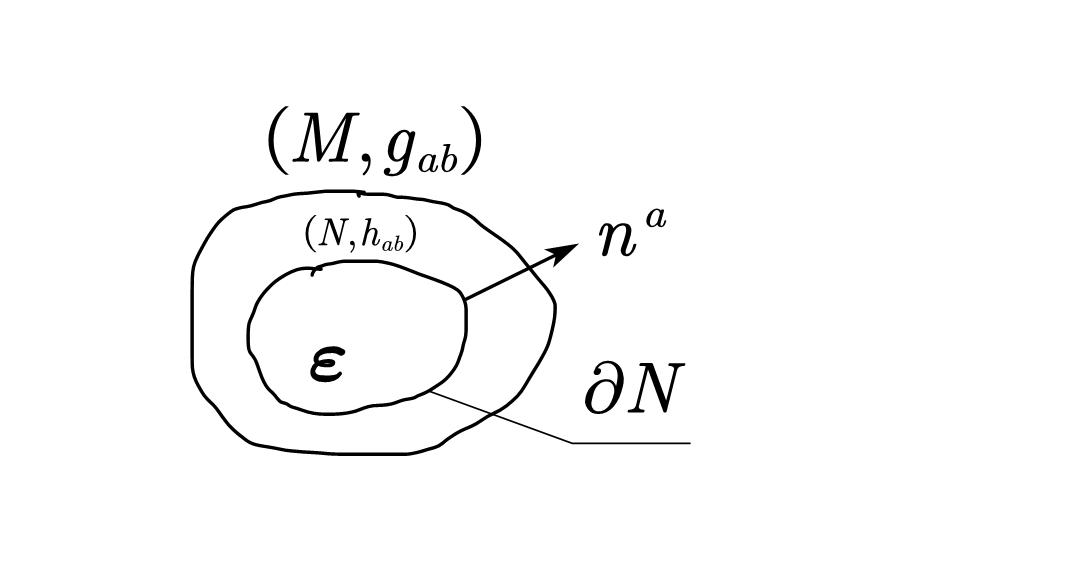
\includegraphics[width=0.8\textwidth]{img/5-6.png}
    \caption{诱导体元,其中$\partial N$非类光超曲面,$n^a$是其归一化法矢}
    \label{fig:5-6}
\end{figure}

如图\ref{fig:5-6}所示,$\partial N$非类光超曲面,$n^a$是其归一化法矢,满足$n^an_a=\pm 1.N$上的度规$g_{ab}$在$\partial N$上的诱导度规为$h_{ab}=g_{ab}\mp n_an_b .$将$\partial N$视为带度规$h_{ab}$的$n-1$维流形,其体元$\hat{\varepsilon}_{a_1\cdots a_n}$满足:
\begin{itemize}
    \item 与$\partial N$的诱导定向$\overline{\varepsilon}_{a_1\cdots a_{n-1}}$相容;
    \item 与度规相容,即$$\hat{\varepsilon}^{a_1\cdots a_{n-1}}\hat{\varepsilon}_{a_1\cdots a_{n-1}}=(-1)^{\hat{s}}(n-1)!,$$
    其中$\hat{\varepsilon}^{a_1\cdots a_{n-1}}$是$h^{ab}$对$\hat{\varepsilon}_{a_1\cdots a_{n-1}}$升指标的结果,$\hat{s}$为$h_{ab}$中负数对角元的个数.
    
    $\partial N$上满足如上两个条件的体元$\hat{\varepsilon}_{a_1\cdots a_{n-1}}$称为\textcolor{blue}{诱导体元}.
\end{itemize}
\newpage
设$M$是$n$维定向流形,$N$是$M$中的$n$维紧致带边嵌入子流形,$g_{ab}$是$M$上的度规,$\boldsymbol{\varepsilon},\nabla_a$分别是适配体元和适配导数算符,$\hat{\boldsymbol{\varepsilon}}$是$\partial N$上的诱导体元,$\partial N$的外法矢$n^a$满足$n^an_a=\pm 1$,$v^a$是$M$上的$C^1$矢量场,则有
\begin{align}
    \boxed{\int_{\text{i}(N)}(\nabla_av^a)\boldsymbol{\varepsilon}=\pm \int_{\partial N}v^an_a\hat{\boldsymbol{\varepsilon}}.}
\end{align}
\begin{proof}
    由于$$
    \int_{\text{i}(N)}(\nabla_bv^b)\boldsymbol{\varepsilon}=\int_{\partial N}v^b\varepsilon_{ba_1\cdots a_{n-1}}=\int_{\partial N}\tilde{\boldsymbol{\omega}},
    $$
    只要证$$\tilde{\omega}_{a_1\cdots a_{n-1}}=\pm v^bn_b
   \hat{\boldsymbol{\varepsilon}},
    $$
    上式两边都是$n-1$形式,故必存在$K$使得
    $$
    \tilde{\omega}_{a_1\cdots a_{n-1}}=K v^bn_b
   \hat{\varepsilon}_{a_1\cdots a_{n-1}}.
    $$
只要证明$K=\pm 1.$
    
设$\{(e_0)^a=n^a,(e_1)^a,\cdots,(e_{n-1})^a\}$是$V_q$的一个右手正交归一基底,对上式左右两边作用$(e_1)^a\cdots (e_{n-1})^a$,
    $$
    \text{右边}=Kv^bn_b\hat{\varepsilon}_{12\cdots (n-1)}=\pm Kv^b(e^0)_b=\pm Kv^0;
 $$
 $$
    \begin{aligned}
        \text{左边} &=\omega_{a_1\cdots a_{n-1}}(e_1)^{a_1}\cdots (e_{n-1})^{a_{n-1}}=v^b\varepsilon_{ba_1\cdots a_{n-1}}(e_1)^{a_1}\cdots (e_{n-1})^{a_{n-1}}\\
    &=v^\mu\varepsilon_{\mu 1\cdots (n-1)}=v^0\varepsilon_{01\cdots(n-1)}=v^0.
    \end{aligned}
    $$
    所以$K=\pm 1.$
\end{proof}

\section{对偶微分形式}
设$\Lambda_p(l)$代表$p\in M$的全部$l$形式的集合($l\leqslant n$),则有
\begin{align}
    \text{dim}\Lambda_p(l)=\dfrac{n!}{l!(n-l)!}=\text{dim}\Lambda_p(n-l).
\end{align}
$\forall \boldsymbol{\omega}\in \Lambda_M(l)$,定义$\boldsymbol{\omega}$的\textcolor{blue}{对偶微分形式}(dual form)$^*\boldsymbol{\omega}\in \Lambda_M(n-l)$为
\begin{align}
    \boxed{^*\omega_{a_1\cdots a_{n-l}}:=\dfrac{1}{l!}\omega^{b_1\cdots b_l}\varepsilon_{b_1\cdots b_la_1\cdots a_{n-l}} ,}
\end{align}
其中$*:\Lambda_M(l)\to\Lambda_M(n-l)$为同构映射.

$f$作为0形式场,其对偶微分形式为
\begin{align}
    (^*f)_{a_1\cdots a_n}=\dfrac{1}{0!}f\varepsilon_{a_1\cdots a_n}=f\varepsilon_{a_1\cdots a_n},
\end{align}
所以从这一角度出发,可以将函数$f$的积分和$f$的对偶形式场的积分等同.而
\begin{align}
    ^*(^* f)=\dfrac{1}{n!}(f\varepsilon^{b_1\cdots b_n})\varepsilon_{b_1\cdots b_n}=\dfrac{1}{n!}f(\underbrace{\varepsilon^{b_1\cdots b_n}\varepsilon_{b_1\cdots b_n}}_{(-1)^sn!})=(-1)^sf.
\end{align}

为什么在三维欧氏空间中无需使用微分形式和对偶微分形式?
\begin{itemize}
\item 在三维欧氏空间中,利用欧式度规$\delta_{ab}$可以将对偶矢量场$\omega_a$变为矢量场$\omega^a=\delta^{ab}\omega_{b}$,从而无需使用1形式场.
\item 由于维度为3,同构映射$^*:\Lambda_{M}(2)\to\Lambda_M(1)$使得$\omega\in \Lambda_M(2)$和$^*\omega\in \Lambda_M(1)$等同,从而无需使用2形式场.
\item 同构映射$^*:\Lambda_{M}(3)\to\Lambda_M(0)$使得$\omega\in \Lambda_M(3)$和$^*\omega\in \Lambda_M(0)$等同,从而无需使用3形式场.
\end{itemize}

所以三维欧氏空间的微分形式场都可以用函数和矢量场代替.

对于三维空间中的矢量$\boldsymbol{A},\boldsymbol{B}$,其标量积用微分几何的语言可以表述为
\begin{align}
    \boldsymbol{A}\cdot \boldsymbol{B}=\delta_{ab}A^aB^b,
\end{align}

由于
$$
\begin{aligned}
\omega_{ab}&\equiv A_a\wedge B_b=2A_{[a}B_{b]}\Rightarrow \omega^{ab}= 2A^{[a}B^{b]},\\
(^*\omega)_c&\equiv\dfrac{1}{2}\omega^{ab}\varepsilon_{abc}=\varepsilon_{abc}A^aB^b,
\end{aligned}
$$
所以有
$$
(^*\omega)_k=\varepsilon_{ijk}A^iB^j=(\boldsymbol{A}\times\boldsymbol{B})_k,
$$
所以矢量积$\boldsymbol{A}\times \boldsymbol{B}$可以视为先求其楔形积$\boldsymbol{A}\wedge\boldsymbol{B}$,再求其对偶形式,即$\times =*\circ \wedge$,
\begin{align}
    (\boldsymbol{A}\times \boldsymbol{B})_k=\varepsilon_{ijk}A^iB^j,
\end{align}
其中,$\varepsilon_{ijk}$是与欧式度规$\delta_{ab}$适配体元$\varepsilon_{abc}$的分量,而且在笛卡尔系下正交归一,这就是所谓的Levi-Civita记号.

使用微分几何的语言改写三维欧氏空间中矢量场论的若干结论如下:
\begin{enumerate}
\item $\nabla f=\partial_a f$;
\item $\nabla \cdot \boldsymbol{A}=\partial_a A^a$;
\item $\nabla \times \boldsymbol{A}=\varepsilon^{abc}\partial_aA_b$;
\item $\text{grad}f=\text{d}f$;
\item $\text{div}\boldsymbol{A}=^*(\text{d}^*\boldsymbol{A})$;
\item $\text{curl}\boldsymbol{A}=^*(\text{d}\boldsymbol{A})$;
\item $\displaystyle \oint\boldsymbol{E}\cdot \text{d}\boldsymbol{l}=0\Leftrightarrow\text{curl} \boldsymbol{E}=0\Rightarrow \exists \phi \ s.t. \boldsymbol{E}=\nabla \phi;$
\item $\displaystyle \oiint \boldsymbol{B}\cdot \text{d}\boldsymbol{s}=0\Leftrightarrow \text{div}\boldsymbol{B}=0\Rightarrow \exists \boldsymbol{A}\ s.t. \boldsymbol{B}=\text{curl}\boldsymbol{A}.$
\end{enumerate}
\begin{proof}
    结论7和8的证明如下:
    $$
    \begin{aligned}
       & \text{curl}\boldsymbol{E}=0\Leftrightarrow^*(\text{d}\boldsymbol{E})=0\Rightarrow\text{d}\boldsymbol{E}=0\stackrel{\mathbb{R}^3}{\Longrightarrow}\exists \phi \ s.t. \boldsymbol{E}=\nabla \phi;\\
    &\text{div}\boldsymbol{B}=0\Leftrightarrow \text{d}^*\boldsymbol{B}=0\Rightarrow \exists \boldsymbol{A}\ s.t. ^*\boldsymbol{B}=\text{d}\boldsymbol{A}\Rightarrow \boldsymbol{B}=^*(\text{d}\boldsymbol{A})=\text{curl}\boldsymbol{A}.
    \end{aligned}
        $$
    \end{proof}
\chapter{狭义相对论}
\section{4维表述基础}
\subsection{预备知识}
不论是否发生了什么,空间的一点和时间的一瞬的结合就叫一个\textcolor{blue}{事件}(event).全部事件的集合叫\textcolor{blue}{时空}(spacetime).狭义相对论中谈及的\textcolor{blue}{粒子}(particle)是模型化语言,是完全没有大小的点,分为有静质量的粒子(质点)和无静质量的粒子(光子,photon)两类.一个粒子的全部历史由一系列事件组成,因此对应于时空中的一条曲线,称为该粒子的\textcolor{blue}{世界线}(world line),如图\ref{fig:6-1}所示.
\begin{figure}[htbp]
    \centering
 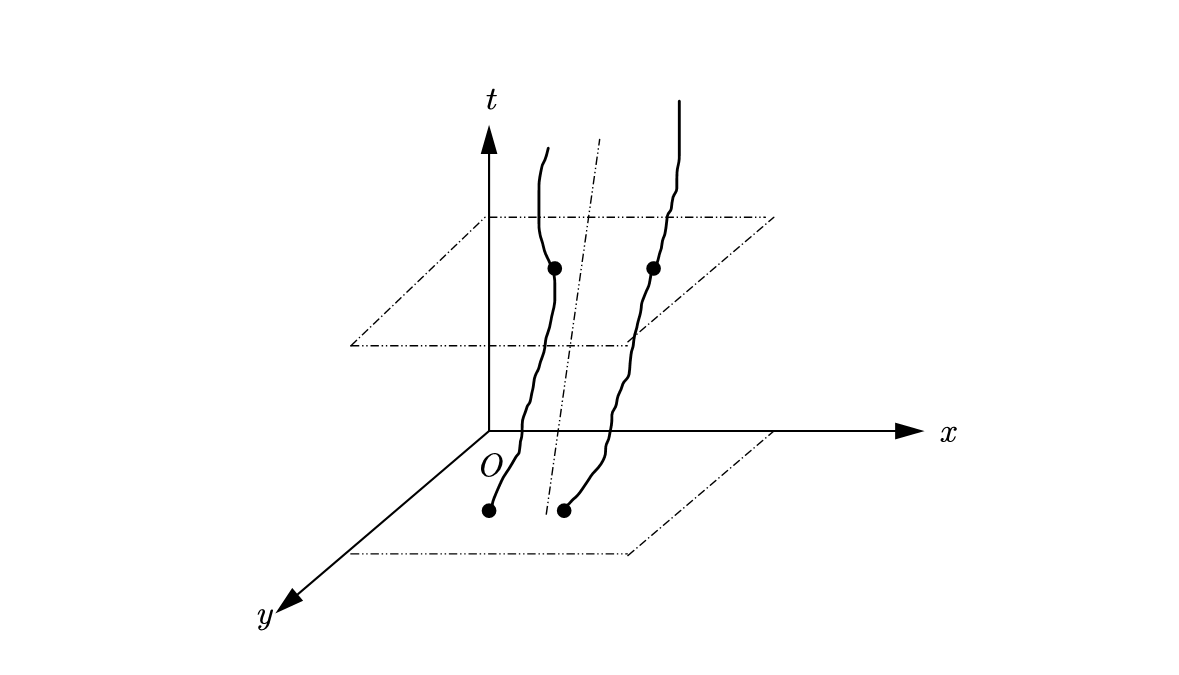
\includegraphics[width=0.8\textwidth]{img/6-1.png}
    \caption{世界线}
    \label{fig:6-1}
\end{figure}

进行物理观测的人叫观察者,将之模型化看成质点,简称\textcolor{blue}{观者}.为了观测,观者手中应有一个走时准确的钟,叫\textcolor{blue}{标准钟}(standard clock),该钟的读数称为该观者的\textcolor{blue}{固有时}(proper time).固有时$\tau$无非是质点世界线的一个特殊参数.
无数观者的集合$\mathscr{R}$叫一个\textcolor{blue}{参考系}(reference frame),满足时空或其一个开子集中的任一点有且仅有$\mathscr{R}$内的一个观者的世界线经过.参考系即世界线的线汇,即对于参考系
\begin{itemize}
\item 过任意事件均有一条世界线.
\item 世界线不相交.
\end{itemize}

\begin{figure}[htbp]
    \centering
 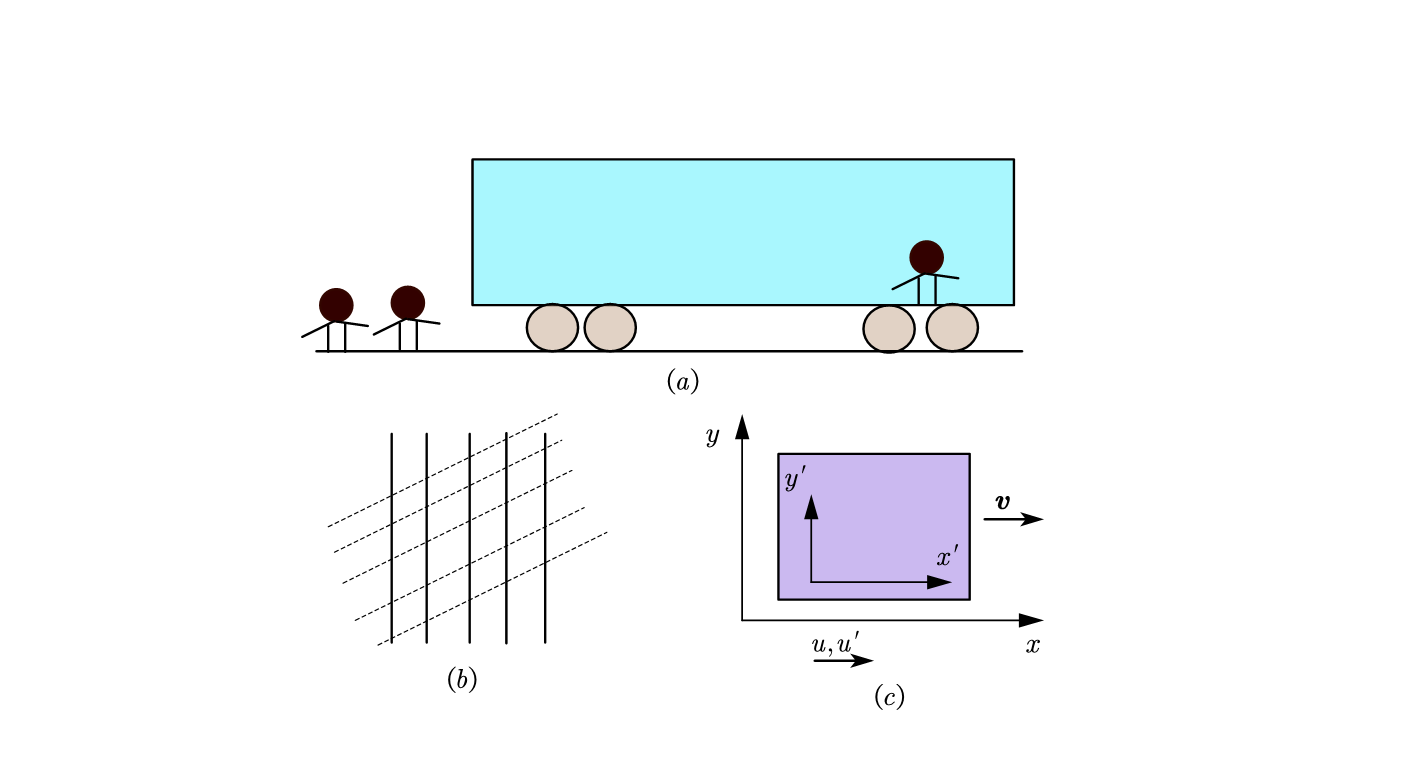
\includegraphics[width=1.2\textwidth]{img/6-2.png}
    \caption{(a):地面系和火车系示意图;(b):地面系(实线)和火车系(虚线)的世界线;(c):Galileo变换}
    \label{fig:6-2}
\end{figure}

如上图\ref{fig:6-2}所示,(a)代表火车系和地面系,而(b)中以许多竖直实线代表地面系观者们的世界线,火车系观者们的世界线则是许多互相平行的斜直虚线.(c)表示Galileo变换,与Galileo相对性原理(任两个惯性系都是平权的)构成Galileo的两大理论贡献.如(c)所示,Galileo变换的坐标变换公式为:
\begin{align}
    \left\{
    \begin{aligned}
        x^\prime&=x-vt\\
        y^\prime&=y\\
        z^\prime&=z\\
        t^\prime&=t
    \end{aligned}
    \right.
\end{align}
坐标变换公式中最后一式蕴含了同时性的绝对性.速度合成公式为:
\begin{align}
    \boldsymbol{u}^\prime=\boldsymbol{u}-\boldsymbol{v}.
\end{align}
\subsection{Maxwell方程的参考系问题}
Maxwell方程组表明Galileo相对性原理对于电磁理论并不成立.于是存在以下两种非此即彼的选择:
\begin{itemize}
\item 认为相对性原理并不总是成立的,即惯性系不平权.存在一个特殊的惯性系(以太,ether),其中光速为c,而其他惯性系则不然.
\item 坚持相对性原理总是成立的.
\end{itemize}

\begin{figure}[htbp]
    \centering
 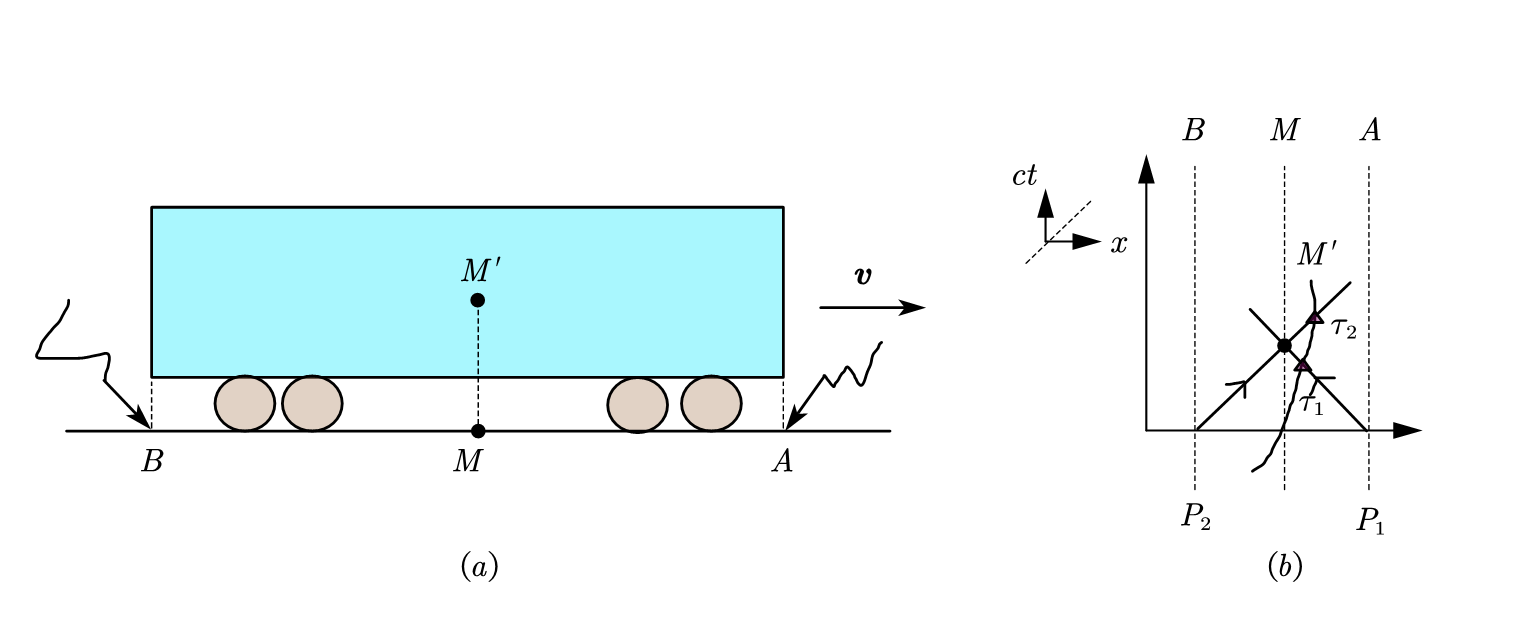
\includegraphics[width=\textwidth]{img/6-3.png}
    \caption{(a):闪电击中车头和车尾;(b):利用世界线进行分析}
    \label{fig:6-3}
\end{figure}


% ------------------------------------------------------------------------------
% Reference and Cited Works
% ------------------------------------------------------------------------------

\bibliographystyle{IEEEtran}
\bibliography{References.bib}

% ------------------------------------------------------------------------------
\cite{1}
\end{document}
